\input{preamble.tex}

\title{Отчет по лабораторной работе № 14. \\ Статическая маршрутизация в Интернете. Настройка}
\author{Сущенко Алина Николаевна\\ НПИбд-01-23}
\date{2026}

\begin{document}

\maketitle
\newpage

\tableofcontents

\newpage
\section{Цель работы}
Настроить взаимодействие через сеть провайдера посредством статической маршрутизации локальной сети организации с сетью основного здания, расположенного в 42-м квартале в Москве, и сетью филиала, расположенного в г. Сочи.

\newpage
\section{Выполнение работы}

\subsection{Настройка связи между площадками}

\subsubsection{Настройка коммутатора ansusenko-sw-1}
В логическую рабочую область проекта добавлен коммутатор \texttt{ansusenko-sw-1}. Выполнена настройка trunk-портов и создание VLAN (Рис. \ref{01}):

\begin{center}
    \centering
    
\includegraphics[width=\textwidth]{../images/01.png}
    \captionof{figure}{Настройка интерфейсов коммутатора ansusenko-sw-1.}
    \label{01}
\end{center}

\subsubsection{Настройка маршрутизатора msk-ansusenko-gw-1}
Выполнена настройка subinterface-ов на маршрутизаторе \texttt{msk-ansusenko-gw-1} для связи с площадками. Создан subinterface f0/1.5 с VLAN 5, IP 10.128.255.1/30, description q42 и subinterface f0/1.6 с VLAN 6, IP 10.128.255.5/30, description sochi (Рис. \ref{02}):

\begin{center}
    \centering
    
\includegraphics[width=\textwidth]{../images/02.png}
    \captionof{figure}{Настройка интерфейсов маршрутизатора msk-ansusenko-gw-1.}
    \label{02}
\end{center}

\subsubsection{Настройка маршрутизатора ansusenko-q42-gw-1}
Выполнена настройка интерфейса для связи с провайдером. Интерфейс f0/1 активирован командой \texttt{no shutdown}, создан subinterface f0/1.5 с IP 10.128.255.2/30, с описанием donskaya (Рис. \ref{03}):

\begin{center}
    \centering
    
\includegraphics[width=\textwidth]{../images/03.png}
    \captionof{figure}{Настройка интерфейсов маршрутизатора ansusenko-q42-gw-1.}
    \label{03}
\end{center}


\subsubsection{Настройка коммутатора sch-ansusenko-sw-1}
Выполнена настройка коммутатора в филиале г. Сочи. Порты f0/23 и f0/24 переведены в режим trunk. Создан VLAN 6 (sochi). Интерфейс Vlan6 активирован (Рис. \ref{04}):

\begin{center}
    \centering
    
\includegraphics[width=\textwidth]{../images/04.png}
    \captionof{figure}{Настройка интерфейсов коммутатора sch-ansusenko-sw-1.}
    \label{04}
\end{center}

\subsubsection{Настройка маршрутизатора sch-ansusenko-gw-1}
Выполнена настройка маршрутизатора в Сочи. Интерфейс f0/0 активирован. Создан subinterface f0/0.6 с IP 10.128.255.6/30, с описанием donskaya (Рис. \ref{05}):

\begin{center}
    \centering
    
\includegraphics[width=\textwidth]{../images/05.png}
    \captionof{figure}{Настройка интерфейсов маршрутизатора sch-ansusenko-gw-1.}
    \label{05}
\end{center}

\subsection{Настройка площадки 42-го квартала}

\subsubsection{Настройка маршрутизатора ansusenko-q42-gw-1}
Выполнена настройка интерфейсов для локальных сетей 42-го квартала. (Рис. \ref{06})

\begin{center}
    \centering
    
\includegraphics[width=\textwidth]{../images/06.png}
    \captionof{figure}{Настройка интерфейсов маршрутизатора ansusenko-q42-gw-1.}
    \label{06}
\end{center}

\subsubsection{Настройка коммутатора ansusenko-q42-sw-1}
Выполнена настройка коммутатора в 42-м квартале (Рис. \ref{07}):

\begin{center}
    \centering
    
\includegraphics[width=\textwidth]{../images/07.png}
    \captionof{figure}{Настройка интерфейсов коммутатора ansusenko-q42-sw-1.}
    \label{07}
\end{center}

\subsubsection{Настройка маршрутизирующего коммутатора ansusenko-hostel-gw-1}
Выполнена настройка маршрутизирующего коммутатора для общежития (Рис. \ref{08}). Созданы:
\begin{itemize}
    \item VLAN 202 (q42-management) с интерфейсом Vlan202 и IP 10.129.1.2/24
    \item VLAN 301 (hostel-main) с интерфейсом Vlan301 и IP 10.129.128.1/24
\end{itemize}

\begin{center}
    \centering
    
\includegraphics[width=\textwidth]{../images/08.png}
    \captionof{figure}{Настройка интерфейсов маршрутизирующего коммутатора ansusenko-hostel-gw-1.}
    \label{08}
\end{center}

\subsubsection{Настройка коммутатора ansusenko-hostel-sw-1}
Выполнена настройка коммутатора общежития (Рис. \ref{09}):

\begin{itemize}
    \item Порт g0/1 переведен в режим trunk
    \item Порт f0/1 переведен в режим access в VLAN 301
    \item Создан VLAN 301 (hostel-main)
    \item Интерфейс Vlan301 активирован
\end{itemize}

\begin{center}
    \centering
    
\includegraphics[width=\textwidth]{../images/09.png}
    \captionof{figure}{Настройка интерфейсов коммутатора ansusenko-hostel-sw-1.}
    \label{09}
\end{center}

\subsection{Настройка площадки в Сочи}

\subsubsection{Настройка маршрутизатора sch-ansusenko-gw-1}
Выполнена настройка subinterface-ов для локальных сетей Сочи (Рис. \ref{10}):
\begin{itemize}
    \item Создан subinterface f0/0.401 с IP 10.130.0.1/24, description sochi-main
    \item Создан subinterface f0/0.402 с IP 10.130.1.1/24, description sochi-management
\end{itemize}

\begin{center}
    \centering
    
\includegraphics[width=\textwidth]{../images/10.png}
    \captionof{figure}{Настройка интерфейсов маршрутизатора sch-ansusenko-gw-1.}
    \label{10}
\end{center}

\subsubsection{Настройка коммутатора sch-ansusenko-sw-1}
Выполнена настройка коммутатора в Сочи (Рис. \ref{11}):
\begin{itemize}
    \item Порт f0/1 переведен в режим access в VLAN 401
    \item Создан VLAN 401 (sochi-main)
    \item Интерфейс Vlan401 активирован
\end{itemize}

\begin{center}
    \centering
    
\includegraphics[width=\textwidth]{../images/11.png}
    \captionof{figure}{Настройка интерфейсов коммутатора sch-ansusenko-sw-1.}
    \label{11}
\end{center}

\subsection{Настройка статической маршрутизации между площадками}

\subsubsection{Настройка маршрутизатора msk-ansusenko-gw-1}
Выполнена настройка статических маршрутов до сетей Москвы и Сочи (Рис. \ref{12}):
\begin{verbatim}
ip route 10.129.0.0 255.255.0.0 10.128.255.2
ip route 10.130.0.0 255.255.0.0 10.128.255.6
\end{verbatim}

\begin{center}
    \centering
    
\includegraphics[width=\textwidth]{../images/12.png}
    \captionof{figure}{Настройка маршрутизации на msk-ansusenko-gw-1.}
    \label{12}
\end{center}

\subsubsection{Настройка маршрутизатора ansusenko-q42-gw-1}
Выполнена настройка маршрута по умолчанию (Рис. \ref{13}):

\begin{verbatim}
ip route 0.0.0.0 0.0.0.0 10.128.255.1
\end{verbatim}

\begin{center}
    \centering
    
\includegraphics[width=\textwidth]{../images/13.png}
    \captionof{figure}{Настройка маршрута по умолчанию на ansusenko-q42-gw-1.}
    \label{13}
\end{center}

\subsubsection{Настройка маршрутизатора sch-ansusenko-gw-1}
Выполнена настройка маршрута по умолчанию (Рис. \ref{14}):
\begin{verbatim}
ip route 0.0.0.0 0.0.0.0 10.128.255.5
\end{verbatim}

\begin{center}
    \centering
    
\includegraphics[width=\textwidth]{../images/14.png}
    \captionof{figure}{Настройка маршрута по умолчанию на sch-ansusenko-gw-1.}
    \label{14}
\end{center}

\subsection{Настройка маршрутизации на 42 квартале}

\subsubsection{Настройка маршрутизатора ansusenko-q42-gw-1}
Выполнена настройка маршрута до сети общежития (Рис. \ref{15}):
\begin{verbatim}
ip route 10.129.128.0 255.255.128.0 10.129.1.2
\end{verbatim}

\begin{center}
    \centering
    
\includegraphics[width=\textwidth]{../images/15.png}
    \captionof{figure}{Настройка маршрута до сети общежития.}
    \label{15}
\end{center}

\subsubsection{Настройка маршрутизирующего коммутатора ansusenko-hostel-gw-1}
Выполнена настройка IP-маршрутизации и маршрута по умолчанию (Рис. \ref{16}):
\begin{verbatim}
ip routing
ip route 0.0.0.0 0.0.0.0 10.129.1.1
\end{verbatim}

\begin{center}
    \centering
    
\includegraphics[width=\textwidth]{../images/16.png}
    \captionof{figure}{Настройка маршрутизации на ansusenko-hostel-gw-1.}
    \label{16}
\end{center}

\subsection{Настройка NAT на маршрутизаторе msk-ansusenko-gw-1}

Выполнена настройка NAT для трансляции адресов внутренних хостов (Рис. \ref{17}):
\begin{itemize}
    \item Интерфейсы f0/1.5 и f0/1.6 помечены как \texttt{ip nat inside}
    \item Создан extended access-list \texttt{nat-inet} с разрешением для хостов:
    \begin{itemize}
        \item 10.129.0.200 (q42)
        \item 10.129.128.200 (hostel)
        \item 10.130.0.200 (sochi)
    \end{itemize}
\end{itemize}

\begin{center}
    \centering
    
\includegraphics[width=\textwidth]{../images/17.png}
    \captionof{figure}{Настройка NAT на маршрутизаторе msk-ansusenko-gw-1.}
    \label{17}
\end{center}

\subsection{Проверка корректности настроек}

\subsubsection{Проверка VLAN}
Выполнена проверка VLAN на коммутаторах (Рис. \ref{18}-\ref{20}):

\begin{center}
    \centering
    
\includegraphics[width=\textwidth]{../images/18.png}
    \captionof{figure}{Результат настроек на ansusenko-q42-sw-1.}
    \label{18}
\end{center}

\begin{center}
    \centering
    
\includegraphics[width=\textwidth]{../images/19.png}
    \captionof{figure}{Результат настроек на ansusenko-hostel-sw-1.}
    \label{19}
\end{center}

\begin{center}
    \centering
    
\includegraphics[width=\textwidth]{../images/20.png}
    \captionof{figure}{Результат настроек на sch-ansusenko-sw-1.}
    \label{20}
\end{center}

\subsubsection{Проверка состояния интерфейсов}
Выполнена проверка состояния интерфейсов на маршрутизаторе \texttt{ansusenko-q42-gw-1} (Рис. \ref{21}):

\begin{center}
    \centering
    
\includegraphics[width=\textwidth]{../images/21.png}
    \captionof{figure}{Результат выполнения команды show ip interface brief на ansusenko-q42-gw-1.}
    \label{21}
\end{center}

Выполнена проверка состояния интерфейсов на маршрутизаторе \texttt{sch-ansusenko-gw-1} (Рис. \ref{22}):

\begin{center}
    \centering
    
\includegraphics[width=\textwidth]{../images/22.png}
    \captionof{figure}{Результат выполнения команды show ip interface brief на sch-ansusenko-gw-1.}
    \label{22}
\end{center}

\subsubsection{Проверка VLAN}
Выполнена проверка VLAN на коммутаторе \texttt{ansusenko-sw-1} (Рис. \ref{23}):

\begin{itemize}
    \item VLAN 5 (q42) - active
    \item VLAN 6 (sochi) - active
    \item VLAN 4 (nat) - active
\end{itemize}

\begin{center}
    \centering
    
\includegraphics[width=\textwidth]{../images/23.png}
    \captionof{figure}{Результат выполнения команды show vlan brief на ansusenko-sw-1.}
    \label{23}
\end{center}

Вид нынешнего vlan. (Рис. \ref{24}-\ref{25}):

\begin{center}
    \centering
    
\includegraphics[width=\textwidth]{../images/24.png}
    \captionof{figure}{Результат выполнения команды show vlan brief на аnsusenko-q42-gw-1.}
    \label{24}
\end{center}

\begin{center}
    \centering
    
\includegraphics[width=\textwidth]{../images/25.png}
    \captionof{figure}{Результат выполнения команды show vlan brief на sch-ansusenko-sw-1.}
    \label{25}
\end{center}

\subsubsection{Проверка NAT}
Выполнена проверка NAT-трансляций и статистики на \texttt{msk-ansusenko-gw-1} (Рис. \ref{26}):
\textbf{Результаты проверки NAT:}
\begin{itemize}
    \item Всего трансляций: 6 (6 static, 0 dynamic, 6 extended)
    \item Inside Interfaces: f0/0.3, f0/0.101-104, f0/1.5, f0/1.6
    \item Outside Interfaces: f0/1.4
    \item Hits: 0, Misses: 250
    \item Пул main-pool: 198.51.100.2 — 198.51.100.14 (13 адресов)
\end{itemize}

Статические NAT-трансляции настроены для серверов:
\begin{itemize}
    \item 198.51.100.10:3389 $\rightarrow$ 10.128.6.200:3389
    \item 198.51.100.2:80 $\rightarrow$ 10.128.0.2:80
    \item 198.51.100.3:20-21 $\rightarrow$ 10.128.0.3:20-21
    \item 198.51.100.4:110,25 $\rightarrow$ 10.128.0.4:110,25
\end{itemize}

\begin{center}
    \centering
    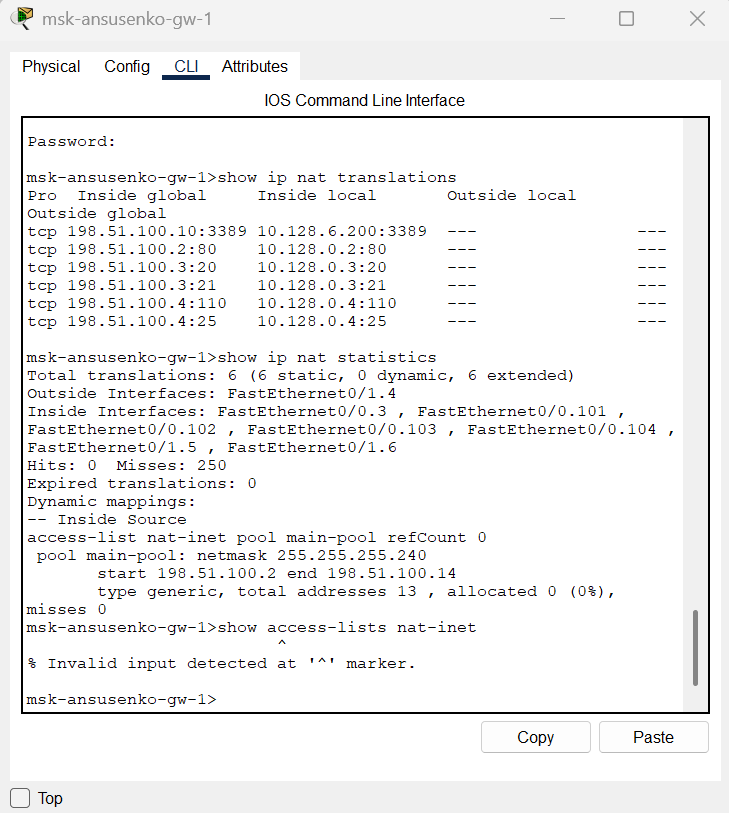
\includegraphics[width=\textwidth]{../images/26.png}
    \captionof{figure}{Результат выполнения команд show ip nat translations и show ip nat statistics.}
    \label{26}
\end{center}

\section{Вывод}

В ходе выполнения лабораторной работы настроена статическая маршрутизация между тремя площадками (провайдер, 42-й квартал в Москве, филиал в Сочи) с использованием технологии VLAN и subinterface-ов. На маршрутизаторах настроены статические маршруты, включая маршруты по умолчанию и суммарные маршруты. На маршрутизаторе msk-ansusenko-gw-1 выполнена настройка NAT для трансляции адресов внутренних хостов.

\end{document}
